\documentclass[12pt, a4paper]{article}
\usepackage[utf8]{inputenc}
\usepackage{polski}
\usepackage{hyperref}
\usepackage{graphicx}
\usepackage{algorithm}
\usepackage{algpseudocode}
\usepackage{amssymb}
\usepackage{geometry}
\usepackage{float}
\usepackage[table]{xcolor}
\title{\textbf{Algorytm ewolucyjny z populacją rosnącą w nieskończoność}}
\author{Adam Stelmaszczyk, Michał Karpiuk}
\date{\today}
\setlength{\parindent}{0in}
\makeatletter\renewcommand{\ALG@name}{}
\renewcommand\refname{Referencje}

\begin{document}
\maketitle

\section{Zadanie}

Celem zadania jest przedstawienie koncepcji, implementacja i testowanie algorytmu ewolucyjnego z populacją rosnącą
w nieskończoność, zawierającą wszystkie punkty wygenerowane do tej pory.

\section{Koncepcja}

Zostanie zaimplementowany algorytm ewolucyjny \cite{jarabas}, dalej nazywany AE, 
działający według schematu \ref{ae}:

\begin{algorithm}[H]
\label{ae}
\begin{algorithmic}[1]
\Function{ae}{}
  \State $T \gets 1$
  \State $P(T) \gets \{x_1, x_2, \ldots, x_n\}$
  \While{$! stop$}
    \For{$i = 0$ \bf{to} $i = n - 1$}
      \State $a \gets$ selekcja$(\{P(1), P(2), \dots, P(T)\}, R)$
      \State $b \gets$ selekcja$(\{P(1), P(2), \dots, P(T)\}, R)$
      \State $O(T,i) \gets$ mutacja$($krzy{\.z}owanie$(a, b))$
    \EndFor
    \State $P(T+1) \gets$ sukcesja$(P(T), O(T))$
    \State $T \gets T+1$
  \EndWhile
\EndFunction
\end{algorithmic}
\end{algorithm}

Rozwiązania $\{x_1, x_2, \ldots, x_n\}$ reprezentowane są jako wektor liczb rzeczywistych długości $D$,
gdzie $D$ to liczba wymiarów. Szukanym optimum jest minimum funkcji celu $f(x)$. $R$ to rozkład prawdopodobieństwa
wybrania jednej populacji, szczegółowo opisany w rozdziale 3.

\subsection{Mutacja}

Mutacja dodaje szum gaussowski o odchyleniu standardowym do każdej współrzędnej wejściowego rozwiązania.

\begin{algorithm}[H]
\begin{algorithmic}[1]
\Function{mutacja}{$x$}
  \For{$i = 0$ \bf{to} $i = D - 1$}
    \State $mutant[i] \gets x[i] + \mathcal{N}(0, 1)$
  \EndFor
\EndFunction
\end{algorithmic}
\end{algorithm}

\subsection{Krzyżowanie}

Krzyżowanie otrzymuje na wejściu dwa rozwiązania rodzicielskie $x_1,x_2$ i~zwraca jedno rozwiązanie potomne. 
Wykorzystano krzyżowanie uśredniające.

\begin{algorithm}[H]
\begin{algorithmic}[1]
\Function{krzy{\.z}owanie}{$x_1, x_2$}
  \For{$i = 0$ \bf{to} $i = D - 1$}
    \State $potomek[i] \gets \frac{x_1[i] + x_2[i]}{2}$
  \EndFor
\EndFunction
\end{algorithmic}
\end{algorithm}

\subsection{Sukcesja}

Sukcesja na wejściu otrzymuje dwie populacje o rozmiarze $n$: aktualną $P$ oraz populację mutantów $O$.
Wyjściem jest jedna populacja o rozmiarze $n$.

\begin{algorithm}[H]
\begin{algorithmic}[1]
\Function{sukcesja}{$P, O$}
  \For{$i = 0$ \bf{to} $i = n - 1$}
    \If{$f(O(T, i)) < f(P(T, i)) $}
      \State $P(T+1, i) \gets O(T, i)$
    \Else
      \State $P(T+1, i) \gets P(T, i)$
    \EndIf
  \EndFor
\EndFunction
\end{algorithmic}
\end{algorithm}

\subsection{Selekcja}

Selekcja otrzymuje na wejściu zbiór wszystkich populacji $X$ oraz rozkład prawdopodobieństwa $R$.
Selekcja najpierw wybiera z prawdopodobieństwem zgodnym z rozkładem $R$ jedną populację z $X$. 
Następnie z tej wybranej populacji losuje i~zwraca jedno rozwiązanie wylosowane zgodnie z rozkładem jednostajnym.
Do generowania losowych indeksów zgodnych z dowolnym dyskretnym rozkładem $R$ wykorzystaliśmy algorytm Inverse Transform \cite{norm}.

\begin{algorithm}[H]
\begin{algorithmic}[1]
\Function{selekcja}{$X, R$}
  \State $P \gets X[R(1, |X|)]$
  \State $wynik \gets P[\mathcal{U}(1, |P|)]$
\EndFunction
\end{algorithmic}
\end{algorithm}

\section{Testowanie}

AE wykorzystujący wszystkie populacje (a nie tylko aktualną) będziemy nazywać NAE - nieskończony algorytm ewolucjny, 
tzn. AE z populacją rosnącą w nieskończoność.
Wersji NAE może być wiele, w zależności od wybranego rozkładu $R$. 
W tej pracy zakładamy, ze funkcja gęstości prawdopodobieństwa rozkładu $R$ jest postaci $at^w + b$, gdzie
$a, b, w \in \mathbb{R_+} \cup \{0\}$ to parametry, zaś $t \in \mathbb{N}$ to numer populacji. 
Porównano następujące algorytmy:

\begin{enumerate}
 \item Klasyczny AE.
 \item NAEU, NAE z rozkładem jednostajnym $\mathcal{U}$, czyli funkcja gęstości prawdopodobieństwa postaci $\frac{1}{b}$. 
 \item NAEP, rozkład o pierwiastkowej funkcji gęstości prawdopodobieństwa postaci $a\sqrt{t}$.
 \item NAEL, rozkład o liniowej funkcji gęstości prawdopodobieństwa postaci $at$.
 \item NAEK, rozkład o kwadratowej funkcji gęstości prawdopodobieństwa postaci $at^2$.
\end{enumerate}

Przyjmując, że jesteśmy w populacji $T = 10$, prawdopodobieństwo wylosowania populacji $t \leq T$ wynosi:
\begin{enumerate}
 \item 1 dla $t=T$, 0 dla $t \neq T$:
  \begin{figure}[H]
  \centering
  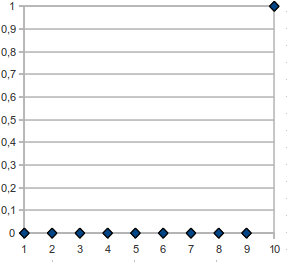
\includegraphics[scale=0.5]{img/1.png} 
  \end{figure}
 \item $\frac{1}{T}$:
  \begin{figure}[H]
  \centering
  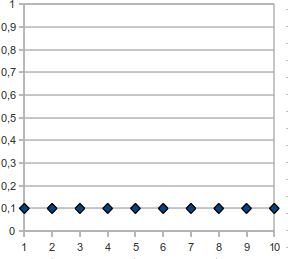
\includegraphics[scale=0.5]{img/2.png} 
  \end{figure}
 \item $\frac{6\sqrt{t}}{(4T+1)\sqrt{T+1}}$
\footnote{Szukamy takiego $a$, dla którego $\sum\limits_{t=1}^T a\sqrt{t} = 1$. Zatem $a = \frac{1}{1 + \sqrt{2} + \dots + \sqrt{T}}$. 
Suma w mianowniku jest równa $\frac{1}{6}(4T+1)\sqrt{T+1}$ z dokładnością do 0,5 \cite{snehal}.}:
  \begin{figure}[H]
  \centering
  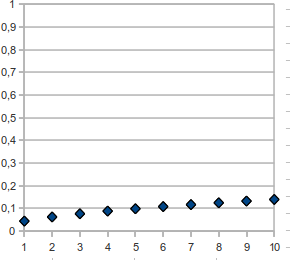
\includegraphics[scale=0.5]{img/3.png} 
  \end{figure}
 \item $\frac{2t}{T(T+1)}$
\footnote{Ponieważ $1 + 2 + \dots + T = \frac{T(T+1)}{2}$.}:
  \begin{figure}[H]
  \centering
  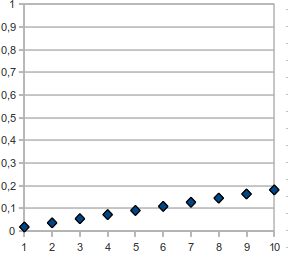
\includegraphics[scale=0.5]{img/4.png} 
  \end{figure}
 \item $\frac{6t^2}{T(T+1)(2T+1)}$
\footnote{Ponieważ $1^2 + 2^2 + \dots + T^2 = \frac{T(T+1)(2T+1)}{6}$.}:
  \begin{figure}[H]
  \centering
  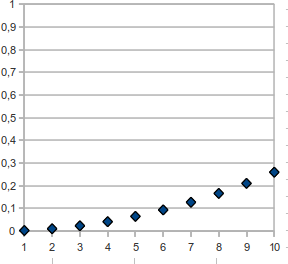
\includegraphics[scale=0.5]{img/5.png} 
  \end{figure}
\end{enumerate}
Eksperymenty przeprowadzono na 7 funkcjach testowych o numerach 15, 16, 19, 20, 21, 22, 24 z BBOB 2013 \cite{finck, hansen}, 
zaimplementowanych w języku C.
Funkcje testowe są wywoływane z Javy, w której napisano algorytmy oraz procedurę testującą.
Liczba wymiarów $D \in \{10, 20, 40\}$. Maksymalna liczba wywołań funkcji oceny $FEs = 10000D$. 
Rozmiar populacji $n = 10D$. 
Na każdej funkcji algorytm był niezależnie uruchamiany 15 razy, z każdego uruchomienia zapisywany był najlepszy wynik.
Jeśli algorytm nie znajdował minimum, wówczas w jednym uruchomieniu, na jednej funkcji, 
generował $\frac{FEs}{n} = 1000$ pokoleń. \\
\\
W NAE zachodzi potrzeba przechowywania $1000$ pokoleń. W najgorszym przypadku, w 40 wymiarach, populacja zawiera 400 rozwiązań.
1 rozwiązanie to wektor 40 zmiennych typu double, zatem około $40\cdot8=320$ bajtów. 
1 populacja zajmuje około $320\cdot400 = 128000$ bajtów $\approx 128$ kB. 
$1000$ populacji zajumuje około $128 \cdot 1000$ kB $\approx 128$ MB. \\
\\
W celu porównania, wykreślano dystrybuanty empiryczne najlepszych wyników z każdego uruchomienia 
algorytmów na jednej funkcji. Najlepszym wynikiem jest najmniejsza różnica funkcji oceny dowolnego rozwiązania od minimum.
Algorytm, którego dystrybuanta na wykresie przebiegała powyżej pozostałych, otrzymywał 4 punkty. 
Za drugie miejsce algorytm otrzymywał 3 punkty, za trzecie 2, za czwarte 1, za ostatnie 0. 
Jeśli dystrybuanty się przecinały, algorytmy zajmowały i-te miejsce ex aequo, a punkty były przyznawane równomiernie.
Dla przykładu, jeśli wszystkie dystrybuanty się przecinały, algorytmy zajmowały ex aequo pierwsze miejsce i otrzymywały po
$\frac{4+3+2+1+0}{5}=2$ punkty.

\nocite{*}
\bibliographystyle{plain}
\bibliography{references}
\end{document}
